\begin{notebox}
\small\textbf{Purpose of this lecture.} Lesson 5 built the general framework --- cryptanalysis vs.\ implementation attacks, passive vs.\ active, and the ``leak, then combine'' recipe --- and used it on ML-KEM's one named riskiest step, split into two concrete attacks. This lecture finishes the job: two attacks on ML-DSA (Dilithium)'s $\vec y$-generation/bound-check step, and two on FN-DSA (Falcon)'s floating-point sampler --- the remaining four of the ``six risky steps'' Lecture 4 promised. We then build one shared countermeasures toolkit covering all three schemes at once, and close with a single map of all six attack surfaces to help you scope your own thesis contribution.
\end{notebox}

\section{ML-DSA, Attack Surface 3: Fault Attacks on Determinism}
\label{sec:L6:fault-attacks-on-determinism}

Recall the factbox from Lecture 4: Dilithium derives its masking vector $\vec y$ \emph{deterministically} from $(sk,\text{msg})$ via a PRF, precisely to avoid the classical failure mode where an accidentally-reused $\vec y$ across two signatures lets an attacker subtract the two signing equations and isolate $\vec s_1$ directly. Determinism kills the \emph{accidental} version of that bug. It does not kill the \emph{deliberate} one.

\begin{rmkbox}{How a Fault Forces Reuse}
$\vec y$ is computed from $(sk,\text{msg})$ by a PRF, then never touched again during that signing call. A fault --- a voltage or clock glitch timed to hit the PRF call, or a skipped instruction that leaves a stale register from a previous signing operation in place --- can make the device use the \emph{same} $\vec y$ for two different messages, without the signer's software ever noticing anything went wrong. Both signatures still verify correctly; nothing about the output looks broken.
\end{rmkbox}

\begin{exbox}{Recovering $s_1$ From Two Faulted Signatures, $q=17$ (Verified by Hand)}
Reuse Lecture 4's exact toy instance: $R_{17}=\mathbb{Z}_{17}[x]/(x^4+1)$, $A=3+5x+2x^2+x^3$, secret $s_1=1$ (unknown to the attacker). The legitimate first signature, exactly as Lecture 4 computed it: mask $y=x$, challenge $c_1=1$, response
$$
z_1 = y+c_1 s_1 = x+1\cdot 1 = 1+x.
$$
Now suppose a fault forces the \emph{same} $y=x$ to be reused when signing a second, different message, whose Fiat--Shamir challenge comes out as $c_2=2$ (different message $\Rightarrow$ different hash input $\Rightarrow$ a different challenge, even with $w=Ay$ unchanged). The second response:
$$
z_2 = y+c_2 s_1 = x+2\cdot 1 = 2+x.
$$
The attacker sees only the two public signatures, $(z_1,c_1)=(1+x,\,1)$ and $(z_2,c_2)=(2+x,\,2)$ --- never $y$ or $s_1$ directly. Subtract:
$$
z_1-z_2 = (1+x)-(2+x) = -1 \equiv 16 \pmod{17}, \qquad c_1-c_2 = 1-2=-1\equiv16\pmod{17}.
$$
Since $z_1-z_2 = (y+c_1s_1)-(y+c_2s_1) = (c_1-c_2)s_1$, the masking term $y$ --- the one thing the attacker never learns directly --- cancels out completely, exactly like Lecture 3's noise-cancellation trick. Solving for $s_1$ (using $(-1)^{-1}\equiv -1\pmod{17}$, since $(-1)\times(-1)=1$):
$$
s_1 = (z_1-z_2)\cdot(c_1-c_2)^{-1} = (-1)\cdot(-1) = 1 \pmod{17} \quad\textbf{--- exactly the true secret.}
$$
This is precisely the calculation Lecture 4's practice exercise asked you to set up symbolically; here it is completed with real numbers, and it recovers the secret in full from just two faulted signatures.
\end{exbox}

\begin{rmkbox}{Why This Is a Complete Break, Not a Partial Leak}
Unlike Section~\ref{sec:L6:fault-attacks-on-determinism}'s sibling attacks in Lesson 5, which needed many queries combined statistically or via a boundary sweep, this one needs exactly \textbf{two} faulted signatures and pure linear algebra --- no averaging, no lattice reduction, no repeated probing. That makes it, coefficient for coefficient, one of the most devastating attacks in this entire two-lesson sequence \emph{when the fault succeeds}: the entire secret $\vec s_1$ falls out in one subtraction. The real engineering difficulty is entirely on the attacker's fault-injection side (precisely timing a glitch to hit the right instruction), not on the algebra --- which is already fully solved, by you, above.
\end{rmkbox}

\section{ML-DSA, Attack Surface 4: Bypassing the Rejection-Sampling Check}
\label{sec:L6:bypassing-rejection-sampling}

Recall from Lecture 4, Section~\ref{sec:L4:why-rejection-sampling-exists-this-is-th}: $\vec z=\vec y+c\vec s_1$ is only \emph{published} if every coefficient stays within an allowed bound; anything outside it is discarded and resampled with fresh $\vec y$. The entire point is that, \emph{conditioned on being published}, $\vec z$'s distribution carries no statistical trace of $\vec s_1$. A fault that skips or corrupts that bound check breaks the conditioning --- without breaking the arithmetic that produced $\vec z$ in the first place.

\begin{rmkbox}{Why Skipping the Check Reveals a Mean Shift}
$\vec y$ is sampled from a range built wide and symmetric around $\vec 0$ specifically so that $\mathbb{E}[\vec y]=\vec 0$. Every legitimate published $z_i = y_i + c s_{1,i}$ therefore has $\mathbb{E}[z_i] = \mathbb{E}[y_i] + cs_{1,i} = cs_{1,i}$ --- a mean shifted by exactly the secret-dependent quantity $cs_{1,i}$. Rejection sampling normally hides this: conditioning on landing inside a window safely \emph{interior} to $y_i$'s full range barely perturbs a symmetric distribution, as long as the shift $cs_{1,i}$ is small relative to the safety margin between the accepted window and $y_i$'s natural spread --- which is exactly why real parameters choose $\vec y$'s range to be comfortably wider than $\vec z$'s allowed bound. \textbf{Bypass the check, and that safety margin no longer matters}: every $z_i$, rejected-in-the-real-scheme or not, gets published, and the raw, unconditioned mean shift $cs_{1,i}$ is sitting right there in the data, waiting to be averaged out.
\end{rmkbox}

\begin{exbox}{A Small Illustration of the Averaging Step}
Suppose an attacker, exploiting a bypassed check, collects five faulted signatures that all happen to share the same challenge $c=1$ (or normalizes each observed $z_i$ by dividing out its own $c$ first), and reads off one coefficient's value each time: $3,\ 5,\ 2,\ 4,\ 3$. The sample average is $(3+5+2+4+3)/5 = 17/5 = 3.4$, already landing close to a true secret coefficient of, say, $s_{1,i}=3$ or $4$. Five samples is far too few for real confidence --- exactly Lesson 5's ``leak a little, combine a lot'' recipe (Lesson 5's Figure~\ref{fig:attack-recipe}) again, this time with the combining step being a literal running average instead of a boundary sweep or an algebraic subtraction. Collecting hundreds or thousands of faulted signatures, exactly as real published attacks on rejection-sampling implementations do, drives the noise down and the estimate of $s_{1,i}$ into certainty.
\end{exbox}

\section{FN-DSA, Attack Surface 5: Sampler Non-Exactness}
\label{sec:L6:sampler-non-exactness}

Recall from Lecture 4, Section~\ref{sec:L4:fn-dsa-falcon-a-different-lattice-a-diff}: Falcon's GPV framework signs by sampling a lattice point from a discrete Gaussian centered near a hashed target, using the trapdoor $(f,g)$ to guide the search. The security argument depends on that sampler being \emph{exact} --- indistinguishable from a true discrete Gaussian, with no data-dependent quirks at all.

\begin{rmkbox}{The Biased-Coin Analogy}
Imagine a coin advertised as fair ($50\%$ heads) that is actually, due to a subtle manufacturing flaw tied to its specific weight distribution, $53\%$ heads. Flip it once, and you learn nothing about the flaw. Flip it a thousand times, and the sample frequency --- roughly $530$ heads instead of $500$ --- reveals the bias clearly, via nothing more than counting. A discrete Gaussian sampler that is subtly \emph{approximate} rather than exact behaves the same way: each individual signature reveals nothing, but the statistical shape of many signatures --- which values get sampled slightly more or less often than a true Gaussian would produce --- can correlate with the specific trapdoor $(f,g)$ that built the sampler, exactly as the coin's bias correlated with its physical flaw.
\end{rmkbox}

\begin{exbox}{A Toy Illustration of Detecting the Bias}
Suppose a correct, exact sampler over $\{-1,0,1\}$ should produce each value with probability $\{0.25,\,0.5,\,0.25\}$ --- a coarse discrete-Gaussian stand-in. A specific flawed implementation, tied to one particular trapdoor, instead produces $\{0.20,\,0.50,\,0.30\}$ --- a small, hard-to-notice skew toward $+1$. An attacker who collects many signatures and tallies the frequency of each sampled value will, over enough signatures, see the count for $+1$ pull measurably above a quarter of the total --- the same counting argument as the biased coin, now applied coefficient by coefficient across many signatures, and correlated against different trapdoor hypotheses to pin down which one produced this specific skew.
\end{exbox}

\section{FN-DSA, Attack Surface 6: Floating-Point Timing and Power Leakage}
\label{sec:L6:floating-point-leakage}

Falcon's fast Fourier sampling is implemented with floating-point arithmetic for speed (Lecture 4's preview box). Floating-point hardware and software are, historically, far harder to make constant-time than the plain integer bound-checks Dilithium's rejection sampling relies on --- and the reason is concrete enough to see directly.

\begin{exbox}{A Toy Floating-Point Leak: Rounding to the Nearest Integer}
A common way to round a floating-point value $x$ to the nearest integer checks its fractional part $f$ against $0.5$:
$$
\texttt{if } f \ge 0.5:\ \texttt{round up} \qquad \texttt{else}:\ \texttt{round down.}
$$
On many real floating-point units, the two branches take measurably different time or power, exactly like Lesson 5's PIN-checker --- except here, the branch outcome doesn't just leak ``was this guess partially right,'' it leaks \textbf{which side of $0.5$ the fractional part of the actual sampled Gaussian value fell on}. That's not a side detail: it's a direct, per-sample bit of the number the trapdoor sampler was supposed to keep hidden. A single signature already involves many such roundings; a full power trace of one signing operation can leak enough of the sampler's intermediate values to reconstruct large parts of $(f,g)$ directly --- which is exactly why \textbf{single-trace} key-recovery attacks (needing only one signature's physical trace, not thousands) are the headline result in Falcon's published attack literature, in sharp contrast to the many-query attacks earlier in this lecture.
\end{exbox}

\begin{rmkbox}{Why This Is Harder to Fix Than It Sounds}
``Just make the rounding constant-time'' undersells the problem. Floating-point units built into real hardware handle rounding, subnormal numbers, and special values (like exactly $0.5$) with timing and power characteristics baked into the silicon --- not something a software patch can fully erase without abandoning hardware floating-point support altogether. Section~\ref{sec:L6:countermeasures-for-all-three-schemes} discusses the real trade-off this forces.
\end{rmkbox}

\section{Countermeasures for All Three Schemes}
\label{sec:L6:countermeasures-for-all-three-schemes}

Lesson 5 introduced constant-time coding and previewed masking for Kyber alone. With all six attack surfaces now on the table, one shared toolkit covers all three schemes --- each technique defends against a different piece of the ``leak, then combine'' recipe.

\begin{rmkbox}{Constant-Time Coding, Scheme by Scheme}
The baseline defense everywhere: make timing and control flow independent of secret data. For \textbf{Kyber}, this means the FO re-encryption comparison (Lesson 5). For \textbf{Dilithium}, it means the rejection-sampling bound check itself must not branch in a way that leaks which coefficients failed --- and, separately, the PRF call generating $\vec y$ must be hardened against the instruction-skip and glitch attacks of Section~\ref{sec:L6:fault-attacks-on-determinism} (redundant computation, glitch detectors, or verifying $\vec y$ was freshly derived before using it). For \textbf{Falcon}, constant-time coding runs into the hardest version of this problem: the real fix usually means replacing floating-point sampling with a carefully designed \textbf{fixed-point or integer-only} sampler, trading some speed for a much smaller, more auditable timing surface --- an active area of implementation research in its own right.
\end{rmkbox}

\begin{rmkbox}{Masking}
Masking splits every secret-dependent value into two or more random shares, computed on separately, so no single physical measurement ever correlates with the secret alone (Lesson 5). Masking Kyber's mod-$q$ arithmetic and compression is already harder than masking a bitwise cipher like AES; masking Dilithium's rejection-sampling comparison adds the extra requirement that the \emph{bound check itself} must be evaluated on shares without ever reconstructing the unmasked value; and masking a \emph{true discrete Gaussian sampler}, as Falcon needs, is harder still and remains an active research problem --- there is no simple, universally agreed-upon masked Gaussian sampler the way there is a masked AES S-box.
\end{rmkbox}

\begin{rmkbox}{Blinding and Shuffling}
Two lighter-weight techniques, often used alongside masking rather than instead of it. \textbf{Blinding} multiplies or adds a single random value to an intermediate computation and removes it later, rather than fully secret-sharing every step --- cheaper than masking, but generally offering a weaker security guarantee. \textbf{Shuffling} randomizes the \emph{order} in which independent operations happen --- which polynomial coefficient gets processed first, say --- so that a power trace can no longer be aligned to a fixed position and averaged cleanly across many traces, directly undercutting the ``combine'' half of the recipe from Lesson 5's Figure~\ref{fig:attack-recipe} without changing what gets computed at all.
\end{rmkbox}

\begin{factbox}{TVLA: How the Field Actually Measures ``Is This Leaking?''}
\textbf{Test Vector Leakage Assessment (TVLA)} is the standard methodology for evaluating whether a given implementation leaks at all, without needing to mount a full key-recovery attack first. The core idea: collect power or EM traces for two carefully chosen sets of inputs (e.g., a fixed secret-dependent value vs.\ a fresh random one each time) and run a statistical test (typically Welch's $t$-test) comparing the two sets, trace point by trace point. A large, consistent statistical difference is evidence of a leak, even if no one has yet turned that leak into a working attack. This is the standard vocabulary you'll want for writing up your own results --- reporting ``no statistically significant leakage detected via TVLA'' is a precise, citable claim, not just ``we didn't find anything.''
\end{factbox}

\section{Bridge to Your Thesis: The Full Six-Surface Picture}
\label{sec:L6:bridge-to-your-thesis}

\begin{figure}[ht]
\centering
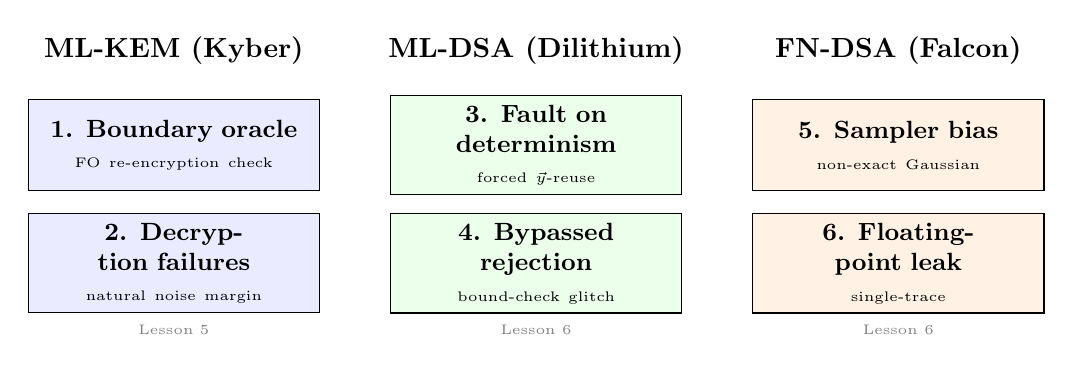
\begin{tikzpicture}[scale=1, every node/.style={font=\small}]
  \node[font=\bfseries] at (0,4.3) {ML-KEM (Kyber)};
  \node[font=\bfseries] at (4.6,4.3) {ML-DSA (Dilithium)};
  \node[font=\bfseries] at (9.2,4.3) {FN-DSA (Falcon)};

  \node[draw, minimum width=3.7cm, minimum height=1.15cm, text width=3.35cm, fill=blue!8, align=center] (k1) at (0,3.1) {\textbf{1. Boundary oracle}\\ \tiny FO re-encryption check};
  \node[draw, minimum width=3.7cm, minimum height=1.15cm, text width=3.35cm, fill=blue!8, align=center] (k2) at (0,1.6) {\textbf{2. Decryption failures}\\ \tiny natural noise margin};

  \node[draw, minimum width=3.7cm, minimum height=1.15cm, text width=3.35cm, fill=green!8, align=center] (d1) at (4.6,3.1) {\textbf{3. Fault on determinism}\\ \tiny forced $\vec y$-reuse};
  \node[draw, minimum width=3.7cm, minimum height=1.15cm, text width=3.35cm, fill=green!8, align=center] (d2) at (4.6,1.6) {\textbf{4. Bypassed rejection}\\ \tiny bound-check glitch};

  \node[draw, minimum width=3.7cm, minimum height=1.15cm, text width=3.35cm, fill=orange!10, align=center] (f1) at (9.2,3.1) {\textbf{5. Sampler bias}\\ \tiny non-exact Gaussian};
  \node[draw, minimum width=3.7cm, minimum height=1.15cm, text width=3.35cm, fill=orange!10, align=center] (f2) at (9.2,1.6) {\textbf{6. Floating-point leak}\\ \tiny single-trace};

  \node[font=\tiny, gray] at (0,0.75) {Lesson 5};
  \node[font=\tiny, gray] at (4.6,0.75) {Lesson 6};
  \node[font=\tiny, gray] at (9.2,0.75) {Lesson 6};
\end{tikzpicture}
\caption{All six attack surfaces from Lessons 5--6, side by side. Every box is one instance of the same recipe as Lesson 5's Figure~\ref{fig:attack-recipe}: find a leak, then combine many observations --- algebraically (surface 3), statistically (surfaces 1, 2, 4, 5), or via a single rich trace (surface 6).}
\label{fig:six-surfaces}
\end{figure}

\begin{previewbox}{A Starting Checklist, Now Covering All Three Schemes}
Extend Lesson 5's Kyber-only checklist with the four questions this lecture adds: (4) Is Dilithium's $\vec y$-derivation hardened against instruction-skip and glitch faults, and does the bound check itself run in constant time? (5) Does a given Falcon implementation's sampler pass a statistical exactness test against a true discrete Gaussian, at a sample size large enough to detect a small bias? (6) Does a power or EM trace of a \emph{single} Falcon signature show detectable, sample-correlated structure around its floating-point rounding operations? As before, a careful, well-documented answer to any one of these six questions --- confirming a leak \emph{or} confirming its absence via TVLA --- is a complete, thesis-worthy floor-level contribution; combining a partial leak from one surface with the lattice-reduction techniques of Lecture 1 to finish a full key recovery is the kind of result that would make a genuinely strong thesis chapter on its own.
\end{previewbox}

\section{Summary Table}
\label{sec:L6:summary-table}

\begin{center}
\renewcommand{\arraystretch}{1.3}
\begin{tabular}{|l|l|l|}
\hline
\textbf{Attack surface} & \textbf{Combine step} & \textbf{Queries needed} \\
\hline
1. Kyber boundary oracle & Algebraic sweep & $O(n\log q)$ \\
2. Kyber decryption failures & Statistical & Many \\
3. Dilithium fault-on-determinism & Algebraic (subtraction) & \textbf{2} \\
4. Dilithium bypassed rejection & Statistical (averaging) & Many \\
5. Falcon sampler bias & Statistical (frequency count) & Many \\
6. Falcon floating-point leak & Single rich trace & \textbf{1} \\
\hline
Constant-time coding & Fixes timing/branch leaks & --- \\
Masking & Fixes value-correlation leaks & --- \\
Blinding, shuffling & Cheaper, weaker alternatives & --- \\
TVLA & Detects leaks before an attack exists & --- \\
\hline
\end{tabular}
\end{center}

\section{Exercises}
\label{sec:L6:exercises}

\begin{exercisebox}{Homework Set}
\begin{enumerate}[leftmargin=*]
  \item Using the same toy Dilithium instance as Section~\ref{sec:L6:fault-attacks-on-determinism}: suppose instead the two observed challenges were $c_1=1$ and $c_2=3$ (still with the same faulted $y=x$). Compute $z_1,z_2$, and confirm the subtraction-and-divide procedure still recovers $s_1=1$.
  \item In your own words (3--4 sentences): why does Attack Surface 3 (Section~\ref{sec:L6:fault-attacks-on-determinism}) need only two signatures while Attack Surface 4 (Section~\ref{sec:L6:bypassing-rejection-sampling}) needs many? Connect your answer to whether each attack's ``combine'' step is algebraic or statistical.
  \item Section~\ref{sec:L6:sampler-non-exactness}'s biased-coin toy used probabilities $\{0.20,0.50,0.30\}$ instead of the correct $\{0.25,0.50,0.25\}$. If an attacker collects $400$ signatures and the sampler is indeed the flawed one, roughly how many times would you expect to see the value $+1$ sampled? How does that compare to what a correct, unbiased sampler would produce over the same $400$ signatures?
  \item Compare Section~\ref{sec:L6:floating-point-leakage}'s single-trace Falcon attack to Lesson 5's Kyber attacks (which need many chosen ciphertexts). In 3--4 sentences, explain why a defender might reasonably treat a single-trace attack as a \emph{more} urgent risk to fix than a many-query attack, even though the many-query attack is, in some sense, more thoroughly demonstrated in the literature.
  \item \textbf{Looking ahead:} using Figure~\ref{fig:six-surfaces} and the checklist in Section~\ref{sec:L6:bridge-to-your-thesis}, write a half-page sketch (this can be genuinely for your own thesis planning, not just a classroom exercise) of which one or two of the six attack surfaces you would prioritize investigating first, and why --- consider available equipment, how well-studied each surface already is in the published literature, and which countermeasure from Section~\ref{sec:L6:countermeasures-for-all-three-schemes} you would evaluate against.
\end{enumerate}
\end{exercisebox}
